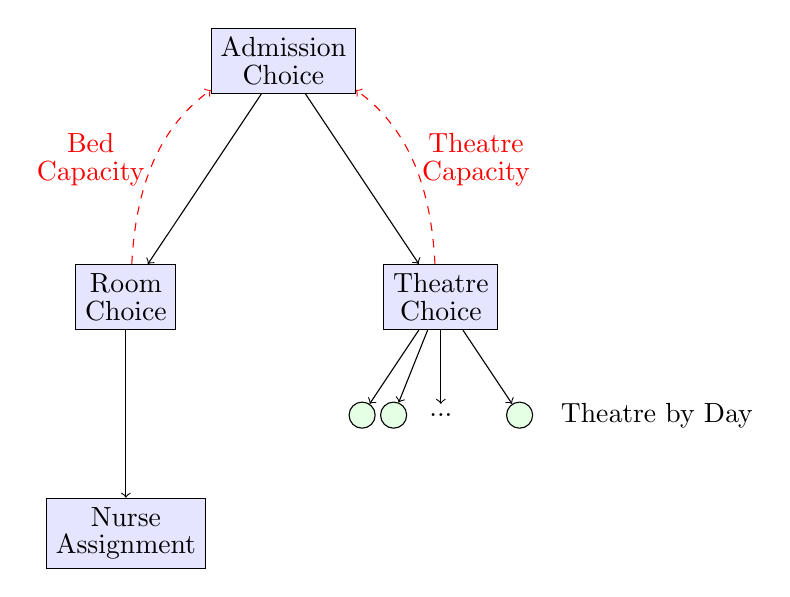
\begin{tikzpicture}[xscale=2,yscale=3]
\node[fill=blue!10,draw=black] (admission) at (2,3) {\shortstack{Admission\\Choice}};
\node[fill=blue!10,draw=black] (theatre) at (3,2) {\shortstack{Theatre\\Choice}};
\node[circle,fill=green!10,draw=black] (d1) at (2.5,1.5) {};
\node[circle,fill=green!10,draw=black] (d2) at (2.7,1.5) {};
\node[draw=none] (dj) at (3,1.5) {...};
\node[circle,fill=green!10,draw=black] (dn) at (3.5,1.5) {};
\node[right,draw=none] () at (3.7,1.5) {Theatre by Day};
\node[fill=blue!10,draw=black] (room) at (1,2) {\shortstack{Room\\Choice}};
\node[fill=blue!10,draw=black] (nurse) at (1,1) {\shortstack{Nurse\\Assignment}};
\draw[->] (admission) -- (theatre);
\draw[->] (admission) -- (room);
\draw[->] (room) -- (nurse);
\draw[->] (theatre) -- (d1);
\draw[->] (theatre) -- (d2);
\draw[->] (theatre) -- (dj);
\draw[->] (theatre) -- (dn);

\draw[red,dashed,->] (theatre) to[bend right] node[right]{\shortstack{Theatre\\Capacity}} (admission);
\draw[red,dashed,->] (room) to[bend left] node[left] {\shortstack{Bed\\Capacity}} (admission);

\end{tikzpicture}
